\section{实轴上的邻域与闭区间}
\label{sec:analysis-metric-measurement}
\label{sec:analysis-set-metric}

前几节的极限都在控制距离：$|a_n-a|<\varepsilon$说明第$n$项离极限不远，
$0<|x-a|<\delta$说明输入离中心不远。下一章研究一元函数的连续性、极值和积分时，还要反复回答三个问题：
“一个点附近”指哪些点；什么样的集合能留住其中点列的极限；
在闭区间每一点附近分别成立的控制，怎样合成对整个区间同时有效的控制。
本节依次用邻域与开闭集、闭集的序列判据和闭区间的有限子覆盖性质回答它们。

\subsection{开球、邻域与开闭集}

\paragraph{开球与邻域}
讨论一个点附近的变化，需要先指定哪些点算作离它足够近。

\begin{definition}[开球与邻域]
\label{def:analysis-open-ball}
设$x\in\mathbb R$，$r>0$。开区间
\[
 B(x,r)=\{y\in\mathbb R:|y-x|<r\}=(x-r,x+r)
\]
称为以$x$为中心、半径为$r$的\term{开球}（open ball）。若集合$V\subseteq\mathbb R$包含某个$B(x,r)$，就称$V$是$x$的邻域。
\end{definition}

在实轴上，开球就是以$x$为中心的对称开区间；用“球”这个名称，是为了后面换成平面或空间中的距离时沿用同一说法。
邻域只要求在$x$周围留出一段余量，本身不必是开区间。例如$[0,1]$是$1/2$的邻域，因为它包含$B(1/2,1/4)$；
它却不是端点$0$的邻域，因为每个$B(0,r)$都含有负数。

\paragraph{开集与闭集}
有了开球，就能检验一个集合是否在其中每个点周围都留有余量；对补集作同样检验，又得到闭集。

\begin{definition}[开集与闭集]
\label{def:analysis-open-closed-sets}
集合$U\subseteq\mathbb R$若对每个$x\in U$都存在$r>0$使$B(x,r)\subseteq U$，就称为\term{开集}（open set）；
集合$F\subseteq\mathbb R$若其补集$\mathbb R\setminus F$为开集，就称为\term{闭集}（closed set）。
\end{definition}

开区间$(a,b)$是开集：对其中的$x$，取$r=\min\{x-a,b-x\}$即可。
闭区间$[a,b]$是闭集，因为补集$(-\infty,a)\cup(b,\infty)$中每一点都能取到不碰到$[a,b]$的小球；
$[a,b]$本身不是开集，端点$a$周围的任何开球都含有区间外的点。
$\mathbb R$与空集既开又闭；但“不是开集”不等于“就是闭集”，例如$[0,1)$在$0$处不开，
它的补集在$1$处也不开，所以$[0,1)$两者都不是。
有限个开集的交仍是开集，可在各点取各个允许半径中最小的一个；无限多个开集的交未必开，
例如$\bigcap_{n\geq1}(-1/n,1/n)=\{0\}$。

\subsection{闭集的序列判据}

闭集由补集定义，使用时却常要问：一列点都在集合中，它的极限是否也在集合中？下面说明这两种说法等价。

\begin{lemma}[闭集的序列判据]
\label{lem:analysis-closed-sequence-criterion}
设$F\subseteq\mathbb R$。$F$是闭集，当且仅当：对每个取值于$F$的数列$(x_n)$，若$x_n\to x$，则$x\in F$。
\end{lemma}
\begin{proof}
若$F$闭而$x\notin F$，开集$\mathbb R\setminus F$包含某个$B(x,r)$。
收敛要求充分靠后的$x_n$落入这个开球，与$x_n\in F$矛盾。
反之，若$F$不闭，则补集不是开集，存在$x\notin F$，使每个$B(x,r)$都与$F$相交。
为每个$n$选$x_n\in F\cap B(x,1/n)$，便有$x_n\to x\notin F$，违反序列条件。
\end{proof}

例如$(0,1)$中的$1/n$趋于$0$，而$0\notin(0,1)$，所以$(0,1)$不是闭集。
闭与有界是不同的性质：$(0,1)$有界但不闭，$\mathbb R$闭但无界。
二者同时成立时，Bolzano--Weierstrass定理~\ref{thm:analysis-bounded-subsequence}给出收敛子列，
本引理又保证子列的极限仍在集合内；下一章的极值定理正是由此得到。

\subsection{闭区间的有限子覆盖性质}

\paragraph{开覆盖与有限子覆盖}

连续性在每一点给出一个邻域内的控制，但不同点的邻域大小可能不同。
要得到对整个闭区间同时有效的结论，需要从无限多个邻域中选出有限个，仍覆盖整个区间。
下面先规定“从一族开集中选出有限部分仍不遗漏”的含义。
\begin{definition}[开覆盖与紧致性]
\label{def:analysis-compactness}
设$K\subseteq\mathbb R$。一族开集的并包含$K$时，称它们为$K$的\term{开覆盖}（open cover）；
从中选出的有限个开集仍覆盖$K$时，称它们构成\term{有限子覆盖}（finite subcover）。
若$K$的每个开覆盖都存在有限子覆盖，则称$K$\term{紧致}（compact）。
\end{definition}
开覆盖本身可以有无限多个成员；有限子覆盖要求从原来的成员中挑选，而不是另换一组集合。

\paragraph{闭区间的紧致性}

闭区间里的点不会逃向无穷，收敛子列的极限也不会离开区间。
这两个条件使局部邻域覆盖不能一直要求加入新的成员。
\begin{theorem}[闭区间的有限子覆盖性质]
\label{thm:analysis-interval-finite-subcover}
实轴上的每个闭区间$[a,b]$都是紧致集。
\end{theorem}
\begin{proof}
$a=b$时选择一个包含该点的覆盖成员即可。设$a<b$，并给定$[a,b]$的开覆盖$\mathcal U$。
先证明这组覆盖有一个共同尺度：
\begin{equation}
 \exists r>0,\quad\forall x\in[a,b],\quad\exists U\in\mathcal U,
 \qquad B(x,r)\cap[a,b]\subseteq U.
\label{eq:analysis-cover-uniform-radius}
\end{equation}
若不存在这样的$r$，对每个$n$可选$x_n\in[a,b]$，使
$B(x_n,1/n)\cap[a,b]$不包含于任何一个覆盖成员。
有界数列$(x_n)$有子列$x_{n_k}\to x\in[a,b]$。
选$U\in\mathcal U$包含$x$，由开性取$\rho>0$使$B(x,\rho)\subseteq U$。
当$k$足够大时，$|x_{n_k}-x|<\rho/2$且$1/n_k<\rho/2$，
于是$B(x_{n_k},1/n_k)\subseteq B(x,\rho)\subseteq U$，产生矛盾。

有了共同半径$r$，把$[a,b]$分成有限个长度小于$r$的小区间。
每段任选一个点$x$，整段都落在$B(x,r)\cap[a,b]$内，故可由一个覆盖成员包含。
每段选择一个这样的成员，得到有限子覆盖。
\end{proof}

每个有界闭集$K\subseteq\mathbb R$也有此性质：先把它放入某个$[a,b]$，
再把$\mathbb R\setminus K$加入它的任意开覆盖，应用闭区间结论后删去这一补集。
有限子覆盖控制的是整个集合，而非只在几个已选点附近留出余量。图~\ref{fig:analysis-process-finite-open-cover}对照一个闭区间的有限覆盖与一个开区间上无法有限选取的覆盖族。
\begin{figure}[!htbp]
 \centering
 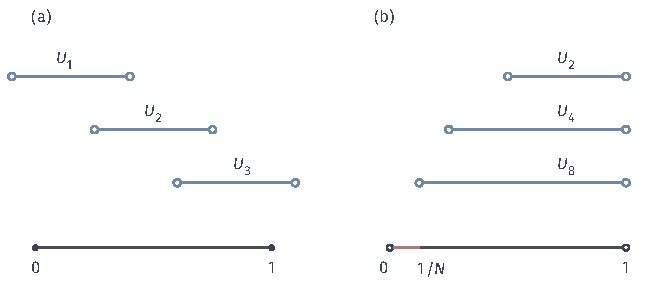
\includegraphics[width=112mm]{figures/01-mathematical-preliminaries-upper/01-mathematical-language-combinatorics-analysis-optimization/tikz/chapter3-concept-processes/finite-open-cover.pdf}
 \caption{(a) 三个开区间$(-0.1,0.4)$、$(0.25,0.75)$、$(0.6,1.1)$覆盖$[0,1]$。(b) $U_n=(1/n,1)$（$n\geq2$）覆盖$(0,1)$；只选有限多个时，设最大下标为$N$，红段$(0,1/N]$仍未覆盖。图只画$U_2,U_4,U_8$；右侧的失败由最大下标论证，不是有限图像的猜测。}
 \label{fig:analysis-process-finite-open-cover}
\end{figure}

以上定义只用到实数之间的距离$|x-y|$。把它换成欧氏距离$\lVert\bm x-\bm y\rVert_2$，
就得到$\mathbb R^d$中的开球$B(\bm x,r)=\{\bm y:\lVert\bm y-\bm x\rVert_2<r\}$、邻域、开集与闭集，
闭集的序列判据连同证明逐字成立；线性空间部分与多元微积分章使用的正是这些欧氏版本。
欧氏空间中闭有界集的子列性质在多元微积分章逐坐标证明，一般距离下的开闭集与紧致性在第~\ref{chap:metric-spaces}章讨论。

\FloatBarrier
